%!TEX root = project.tex

\chapter{System Design}

\section{Log-in System}
When the user starts the program, they are presented with a log-in page. This allows the user to log-in or create a new account.
\newline
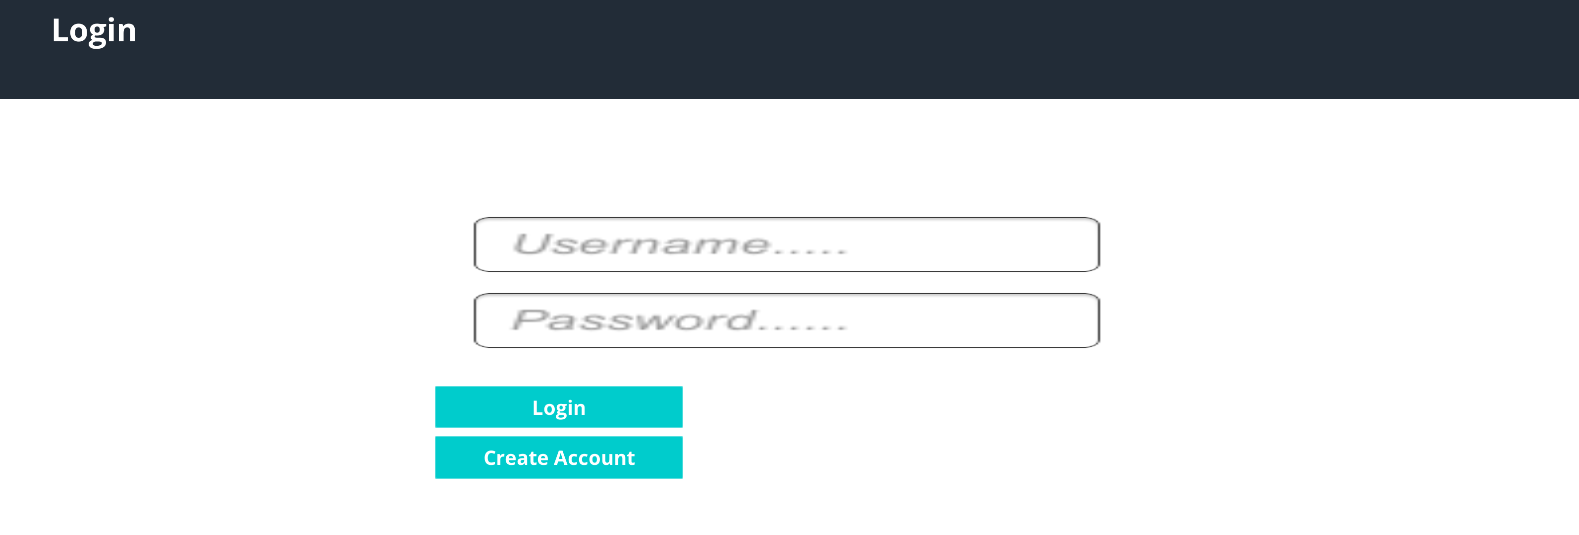
\includegraphics[width=1\columnwidth]{img/LoginActual.PNG}

\section{Hosting a Game}
The user is present with the option to host or join an already hosted game
\newline
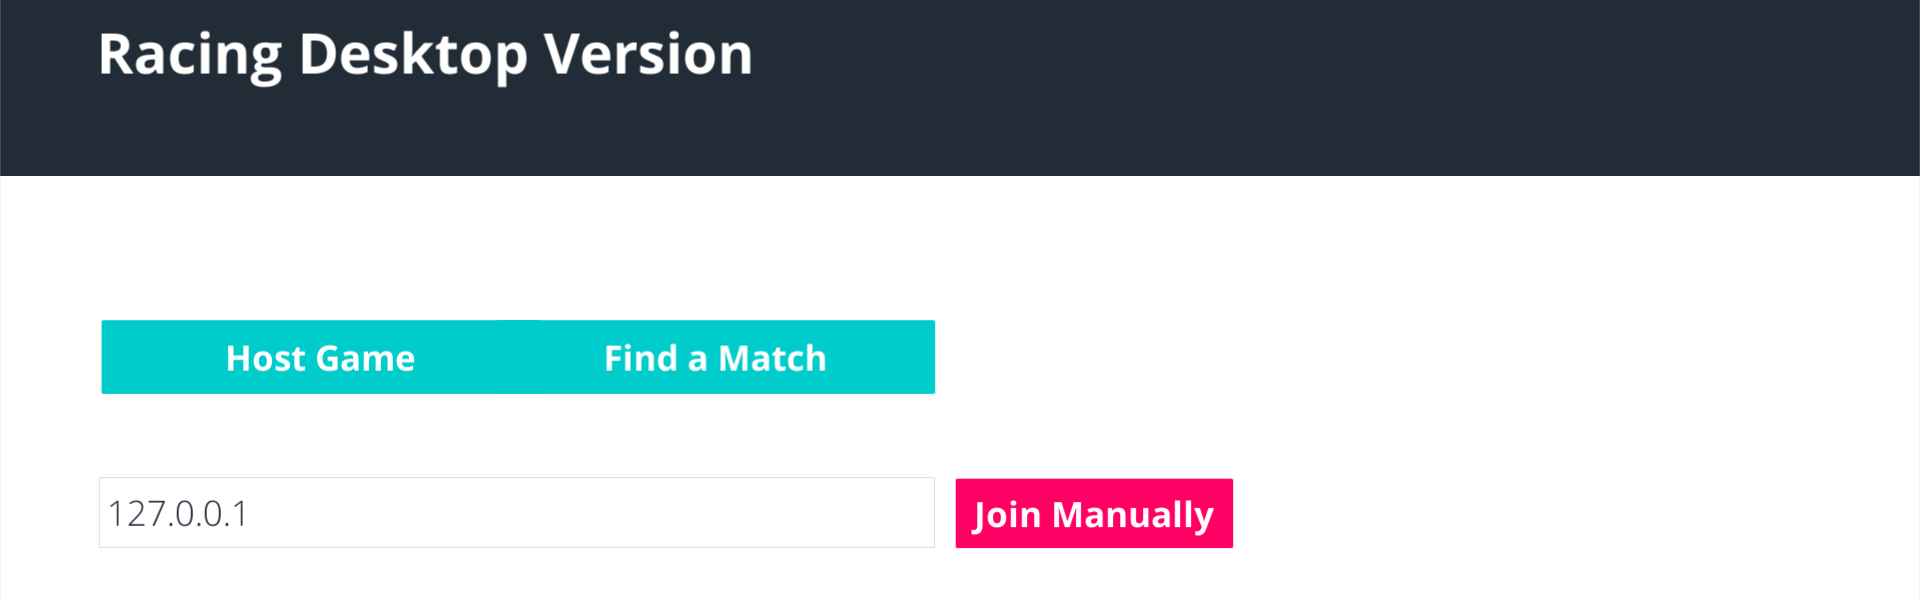
\includegraphics[width=1\columnwidth]{img/MatchFinder1Actual.PNG}

\section{Finding a game}
A list of hosted game is rendered to the screen
\newline
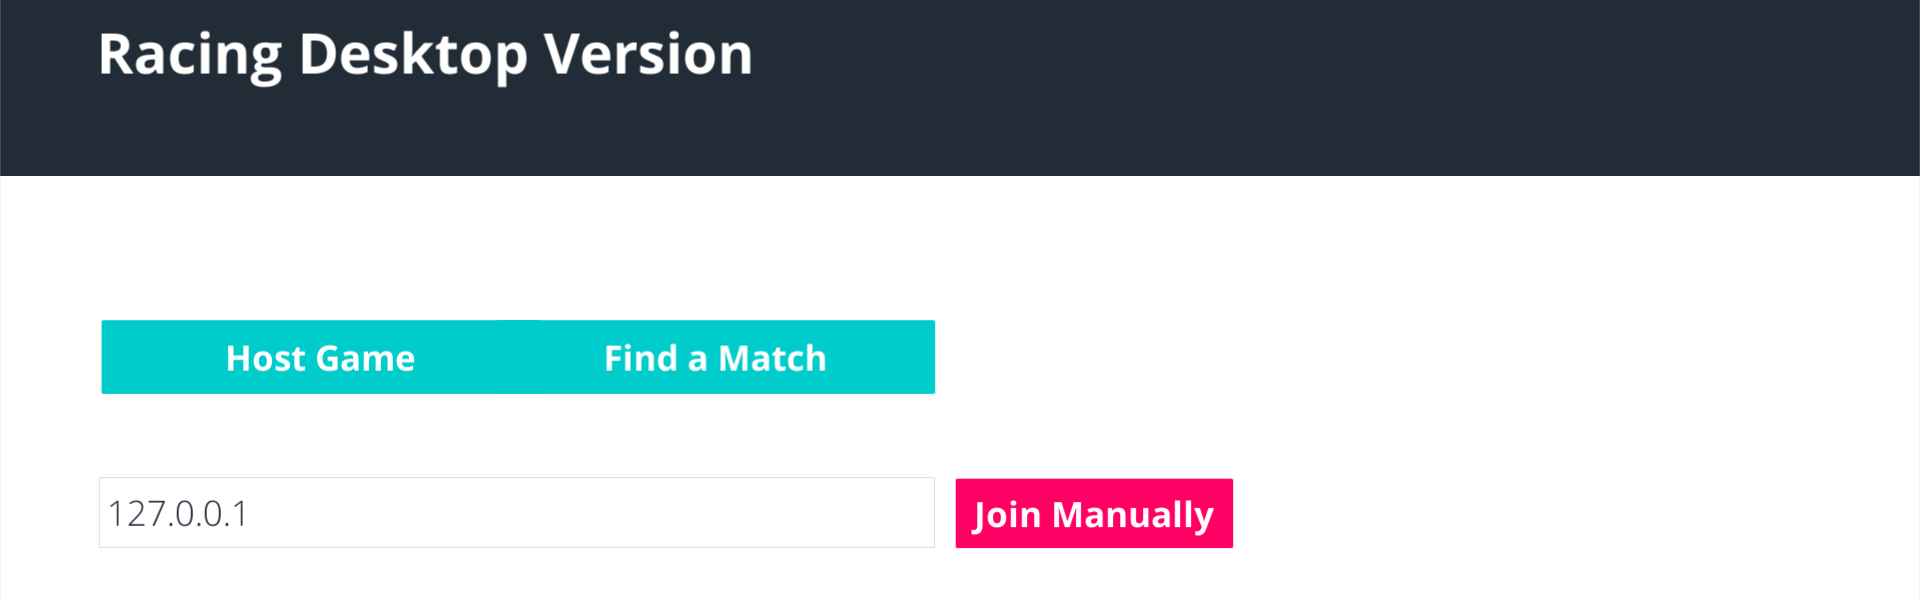
\includegraphics[width=1\columnwidth]{img/MatchFinder1Actual.PNG}

\section{In Game Lobby}
Player came see the player in the game they will be playing
\newline
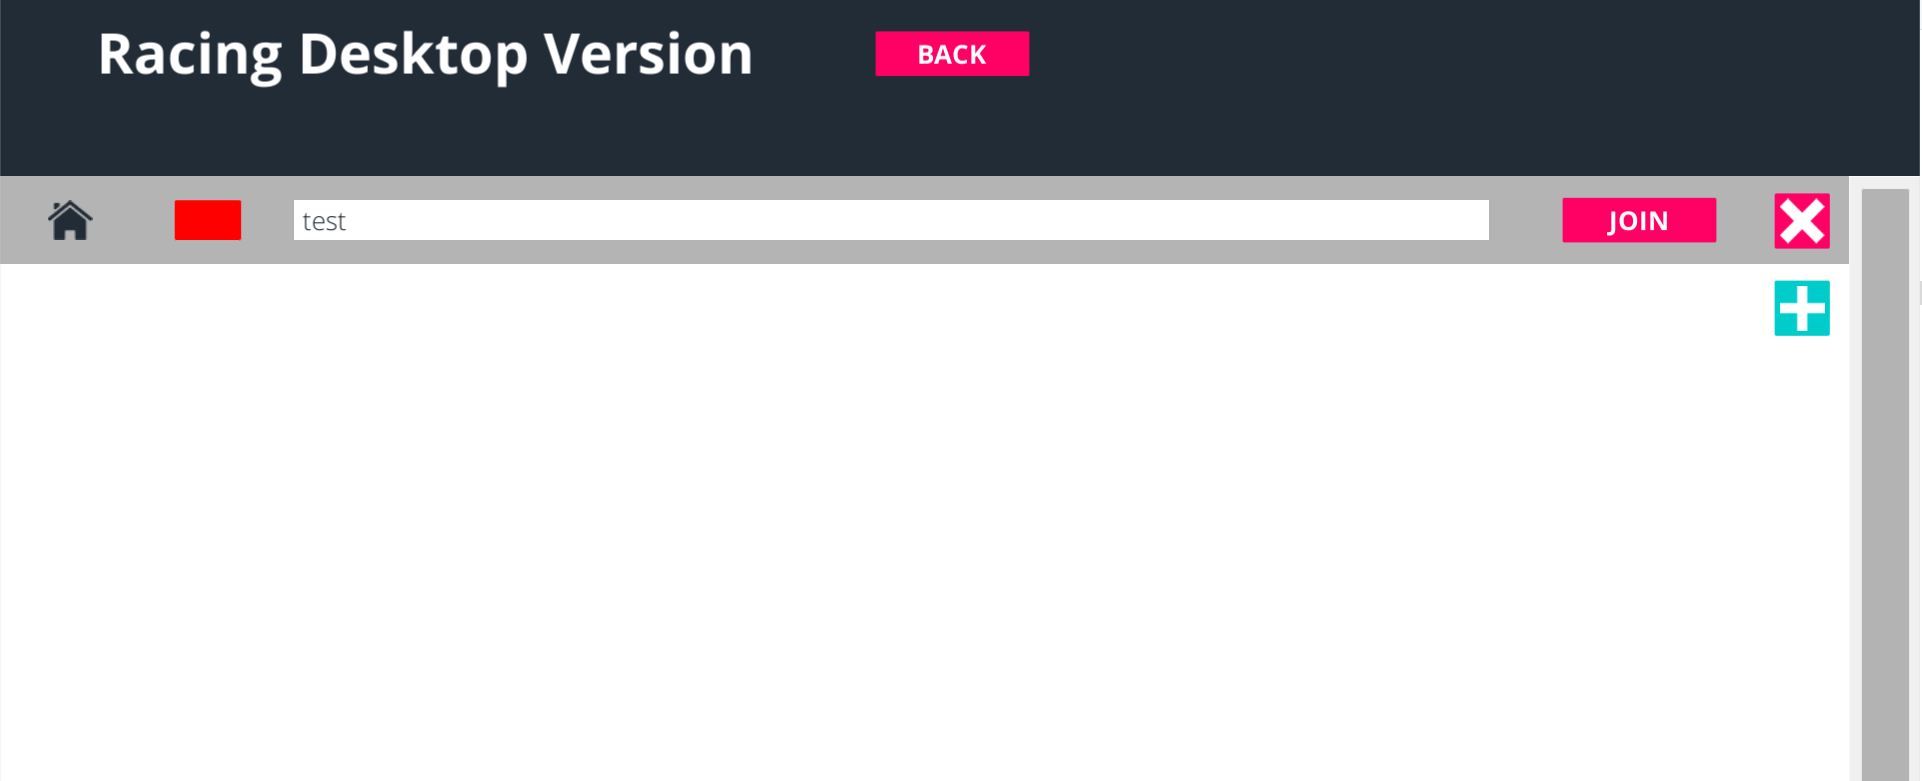
\includegraphics[width=1\columnwidth]{img/LobbyActual.PNG}

\section{The Game on Desktop}

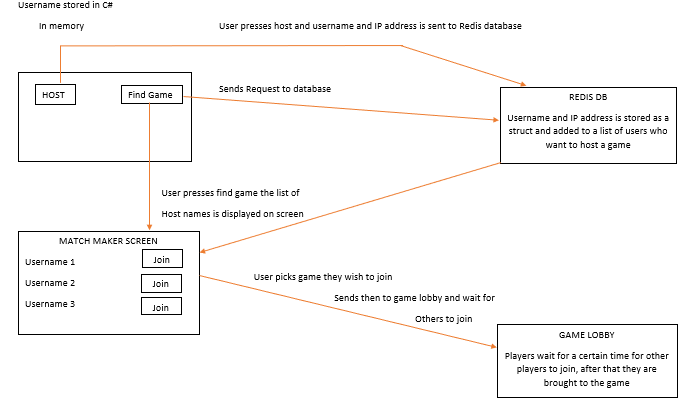
\includegraphics[width=1\columnwidth]{img/redisMatch.PNG}

\section{The Game in Virtual Reality}

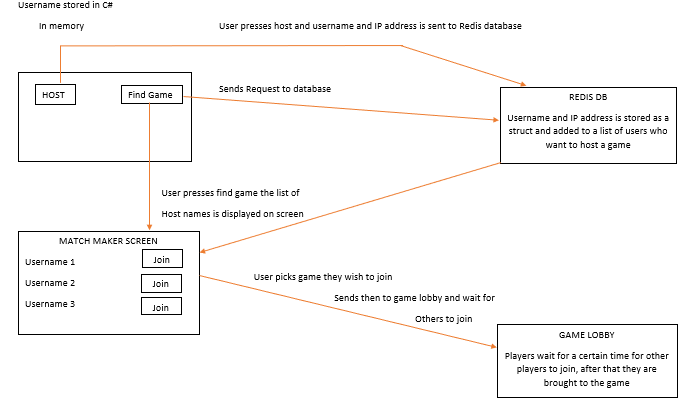
\includegraphics[width=1\columnwidth]{img/redisMatch.PNG}

\section{The Game on a Mobile Device}

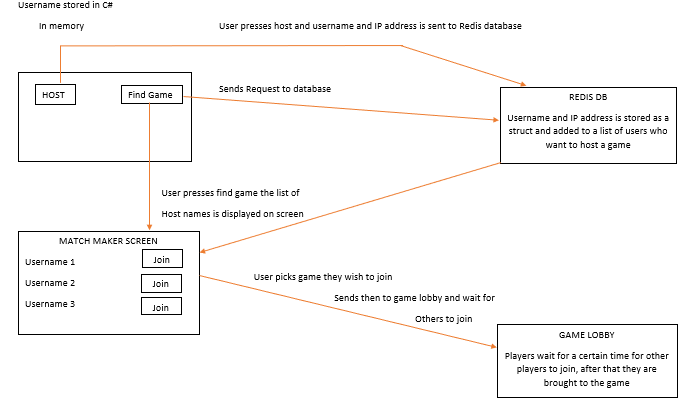
\includegraphics[width=1\columnwidth]{img/redisMatch.PNG}

\section{Scoreboard Screen}

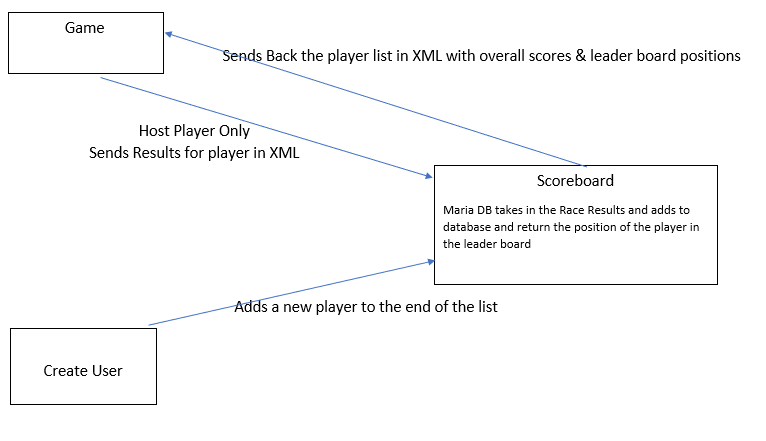
\includegraphics[width=1\columnwidth]{img/scoreBoard.PNG}
The scoreboard is the last window the user will see